%
% Laporan Magang S1 Teknik Elektro
%
% Muhammad Adeel Mahdi Suviyanto (1102183191)
% S1 Teknik Elektro
% Fakultas Teknik Elektro
% Telkom University
%
% Dokumen ini dibuat sesuai dengan kaidah format penulisan Tugas Akhir di Telkom University,
% dengan standar sitasi IEEE.


% Klasifikasi dokumen sebagai report, single column
\documentclass[12pt, a4paper, oneside]{book}

% Load file konfigurasi
%
% Konfigurasi LaTeX Laporan Magang
%
% Muhammad Adeel Mahdi Suviyanto (1102183191)
% S1 Teknik Elektro
% Fakultas Teknik Elektro
% Telkom University
%
%
%

%Data buku
%Judul laporan
\newcommand{\judul}{\textit{BrainDiction}: Aplikasi Android Pendeteksi Tumor Otak Berbasis Machine Learning di Google Cloud Platform}
%Judul laporan, kapital
\newcommand{\JUDUL}{\textit{BRAINDICTION}: APLIKASI ANDROID PENDETEKSI TUMOR OTAK BERBASIS MACHINE LEARNING DI GOOGLE CLOUD PLATFORM}

%Tahun publikasi
\newcommand{\tahun}{2022}
%Tanggal pengesahan
\newcommand{\tanggalpengesahan}{x Juli 2022}

%Data penulis
%Nama penulis
\newcommand{\penulis}{Muhammad Adeel Mahdi Suviyanto}
%Nama penulis, kapital
\newcommand{\PENULIS}{MUHAMMAD ADEEL MAHDI SUVIYANTO}
%NIM
\newcommand{\nim}{1102183191}
%Email penulis
\newcommand{\email}{adeelsuviyanto@gmail.com}
%Program Studi
\newcommand{\prodi}{S1 Teknik Elektro}
%Gelar yang akan diperoleh
\newcommand{\gelar}{Sarjana Teknik}
%Program kuliah
\newcommand{\program}{Teknik Elektro Universitas Telkom}
%Fakultas
\newcommand{\fakultas}{Fakultas Teknik Elektro}
%Fakultas, kapital
\newcommand{\FAKULTAS}{FAKULTAS TEKNIK ELEKTRO}
%Universitas
\newcommand{\universitas}{Universitas Telkom}

%Data Pembimbing
%Pembimbing 1
\newcommand{\pembimbingsatu}{Dr. Eng. Willy Anugrah Cahyadi, S.T, M.T}
\newcommand{\pembimbingdua}{Angga Rusdinar, S.T., M.T., Ph.D.}

%
% Document packages!
%
% Atur sesuai kebutuhan, masih berbasis pada format Proposal Tugas Akhir
%
\usepackage[indonesian]{babel}
\usepackage{amsmath} %Penulisan notasi matematika
\usepackage{amsfonts}
\usepackage{amssymb}
\usepackage{graphicx} %Memasukkan gambar ke laporan
\usepackage{fontenc}
\usepackage{pslatex} %Times New Roman
\usepackage{hyperref}
\usepackage[a4paper, lmargin=4cm, rmargin=3cm, tmargin=3cm, bmargin=3cm]{geometry}
\usepackage[backend=biber, style=ieee, language=english]{biblatex}
\usepackage{csquotes}
\usepackage{fancyhdr} %Header and footer
\usepackage{longtable}
\usepackage{caption} %Caption gambar
\usepackage{setspace}
	\onehalfspacing %Set line spacing ke 1.5
\usepackage[ConnyRevised]{fncychap}
\usepackage{titlesec}
\usepackage{tocloft}
\usepackage{enumitem}
\usepackage{indentfirst}
\usepackage{float}
\usepackage{multirow}
\usepackage[normalem]{ulem}
\useunder{\uline}{\ul}{}
\usepackage{booktabs}
\usepackage{array}
\usepackage{longtable}
\usepackage{lscape}
%
% Chapter style setup
%
\titleformat{\chapter}[display]{\bfseries\large\centering}{BAB \thechapter}{1pt}{}[]
\titlespacing*{\chapter}{0pt}{-50pt}{1.5pt}
%setup section style
\titleformat{\section}[hang]{\bfseries\normalsize}{\thesection \ }{1pt}{}[]
\titlespacing*{\section}{0pt}{0pt}{1.5pt}
\titleformat{\subsection}[hang]{\bfseries\normalsize}{\thesubsection \ }{1pt}{}[]
\titleformat{\subsubsection}[hang]{\bfseries\normalsize}{\thesubsubsection \ }{1pt}{}[]

%set biblatex file
%\addbibresource{./src/ta.bib}

%disable numbering for front matter
\newenvironment{unnumbered}
{\global\chardef\keeplevel=\value{secnumdepth}%
	\setcounter{secnumdepth}{-1}}
{\setcounter{secnumdepth}{\keeplevel}}

%dotted line for TOC
\renewcommand{\cftpartleader}{\cftdotfill{\cftdotsep}} % for parts
\renewcommand{\cftchapleader}{\cftdotfill{\cftdotsep}} % for chapters

% Start dari dokumen
\begin{document}
	
% Cover
\begin{titlepage}
	\begin{center}
	\thispagestyle{empty}
	\textbf{LAPORAN MAGANG}\\
	\bigskip
	\textbf{\JUDUL}\\
	\textbf{PROGRAM BANGKIT ACADEMY 2022}\\
	\bigskip
	\textbf{Periode 12 Februari 2022 - 27 Juli 2022}
	\bigskip
	
	\normalsize
	Disusun sebagai syarat mata kuliah Program Sertifikasi A1, Program Sertifikasi A2, dan Program Sertifikasi A3\\
	Program Studi \prodi
	
	\bigskip
	Disusun oleh:\\
	\textbf{\PENULIS}\\
	\textbf{\nim}\\
	\bigskip
	\bigskip
	\bigskip
	
\includegraphics[scale=0.33]{./assets/logotelu.png}
	\vfill
	\Large
	\textbf{FAKULTAS TEKNIK ELEKTRO}\\
	\large
	\textbf{UNIVERSITAS TELKOM}\\
	\textbf{BANDUNG}\\
	\textbf{2022}
	\end{center} %akhir dari center, mulai dari sini pake subfile
\end{titlepage}

	

% Menyalakan penomoran halaman, angka romawi
\frontmatter
\pagestyle{myheadings}
\setcounter{page}{1}

% Menyalakan section depth numbering
\setcounter{secnumdepth}{5}
	
% Halaman pengesahan
\addcontentsline{toc}{chapter}{LEMBAR PENGESAHAN}
\chapter*{LEMBAR PENGESAHAN} %Lembar Pengesahan sebagai Chapter


\begin{center} %2 halaman pertama all pake center
	\large
	\textbf{LAPORAN MAGANG}
	\bigskip
	
	\Large
	\textbf{\JUDUL}
	\bigskip
	
	\bigskip
	\bigskip
	\bigskip
	
	\normalsize
	\textbf{Telah disetujui dan disahkan sebagai Laporan Magang}\\
	\textbf{Program Studi \prodi}\\
	\textbf{\fakultas}\\
	\textbf{\universitas}\\
	\bigskip
	\bigskip
	
	\textbf{Disusun oleh:}\\
	\textbf{\PENULIS}\\
	\textbf{\nim}\\
	\bigskip
	\bigskip
	
	\textbf{Bandung, 27 Juli 2021}\\
	\begin{tabular}{|p{6cm}|p{6cm}|}
		\hline
		Disusun oleh & Pembimbing Akademik \\
		& \\
		& \\
		& \\
		Muhammad Adeel Mahdi Suviyanto & Angga Rusdinar, S.T., M.T., Ph.D. \\
		\hline
	\end{tabular}
\end{center}



% Halaman pernyataan orisinalitas
\include{./src/orisinalitas}
% Abstrak
\addcontentsline{toc}{chapter}{ABSTRAK}
\chapter*{ABSTRAK}
Bangkit Academy 2022 adalah salah satu program studi independen dari Kampus Merdeka, sebuah program dari Kemendikbudristek yang bertujuan memberikan mahasiswa untuk belajar di luar program studinya di Perguruan Tinggi.  Bekerja sama dengan Google, GoTo, dan Traveloka, Bangkit memberikan kesempatan bagi mahasiswa untuk mendalami ilmu di bidang IT, terutama Google Cloud Platform. Bangkit 2022 dilaksanakan secara daring dan diikuti oleh mahasiswa dari seluruh Indonesia. Dengan metode pembelajaran sinkron dan asinkron, peserta dituntut untuk dapat mengikuti pembelajaran dengan sendiri. Terdapat tiga \textit{learning path} di Bangkit 2022, yakni: \textit{Cloud Computing, Machine Learning,} dan \textit{Android Development}. Pada akhir program Bangkit, seluruh peserta dituntut bekerja secara berkelompok untuk menyelesaikan proyek Capstone membuat sebuah aplikasi Android yang meliputi seluruh elemen pembelajaran dan \textit{learning path} di Bangkit.
% Kata Pengantar
\addcontentsline{toc}{chapter}{KATA PENGANTAR}
\chapter*{KATA PENGANTAR}

Puji syukur kita panjatkan kepada Allah SWT, yang atas rahmat-Nya dan karunianya kami dapat menyelesaikan program Merdeka Belajar - Kampus Merdeka, Bangkit 2022 dengan sukses. Atas karunia-Nya juga, penulis dapat menyelesaikan laporan magang ini dengan tepat waktu.

Pada kesempatan ini penulis juga mengucapkan terima kasih yang sebesar-besarnya kepada pihak Instructor, Facilitator, dan Team dari Bangkit Academy 2022, serta kepada dosen-dosen pengampu program MBKM dari Telkom University atas bantuannya dan bimbingannya dalam menjalani program MBKM Bangkit Academy 2022 ini.

Penulis juga ingin mengucapkan terima kasih kepada keluarga dan teman-teman penulis yang telah memberikan bantuan, doa, bimbingan, dan dukungan kepada penulis hingga akhirnya dapat menyelesaikan program MBKM serta laporan magang ini. Semoga di masa depan penulis dapat membalas amal kebaikan yang diberikan.

\bigskip
\begin{flushright}
	Bandung, 27 Juli 2022\\
	yang menyatakan\\
	\bigskip
	Penulis
\end{flushright}

%Menggunakan angka romawi dalam penomoran bab
\renewcommand{\thechapter}{\Roman{chapter}}
\renewcommand{\thesection}{\arabic{chapter}.\arabic{section}}
\renewcommand{\thesubsubsection}{\arabic{chapter}.\arabic{section}.\arabic{subsection}.\arabic{subsubsection}}
\renewcommand{\thefigure}{\arabic{chapter}.\arabic{figure}}
\renewcommand{\thetable}{\arabic{chapter}.\arabic{table}}
% Daftar isi
\addcontentsline{toc}{chapter}{DAFTAR ISI}
\chapter*{DAFTAR ISI}
\renewcommand*\contentsname{\vspace*{-3cm}}
\tableofcontents
% Daftar gambar
\addcontentsline{toc}{chapter}{DAFTAR GAMBAR}
\chapter*{DAFTAR GAMBAR}
\renewcommand*\listfigurename{\vspace*{-2cm}}
\listoffigures
% Daftar tabel
\include{./src/daftartabel}

% Mulai bagian utama tugas akhir
\mainmatter
% Bab 1
%\chapter{PENDAHULUAN}
\section{Latar Belakang}
Bangkit Academy merupakan sebuah program studi independen oleh Dicoding Indonesia yang bekerja sama dengan Google, GoTo, dan Traveloka. Merupakan bagian dari program Merdeka Belajar Kampus Merdeka oleh Kementerian Pendidikan, Kebudayaan, Riset, dan Teknologi (Kemendikbudristek), peserta Bangkit Academy merupakan mahasiswa aktif semester 5-8 dari seluruh Indonesia dari berbagai program studi.

Sebagai bagian dari program Kampus Merdeka, peserta Bangkit Academy dituntut bertanggung jawab atas pembelajaran modulnya masing-masing, dimana proses belajar-mengajar dilaksanakan secara daring dan ekstra-kampus. Pada tahun 2022, terdapat tiga \textit{learning path} dari program Bangkit Academy, yakni: \textit{Cloud Computing, Machine Learning,} dan \textit{Android Development.}

Proses kegiatan Bangkit Academy terdiri dari beberapa tipe kegiatan: pembelajaran secara sinkron tatap muka, pembelajaran secara asinkron, \textit{capstone project}, dan sertifikasi. Pada Bangkit, peserta juga diajarkan cara berkomunikasi secara profesional, cara memulai karir dan mempersiapkan diri untuk terjun ke dunia kerja, keahlian bisnis, berbahasa Inggris, serta melatih \textit{skill} bekerja sama dengan peserta lainnya.

\section{Lingkup Penugasan}
Lingkup pelaksanaan kegiatan Bangkit 2022 adalah sebagai berikut:
\begin{itemize}
	\item Tanggal: 14 Februari 2022 - 27 Juli 2022
	\item Tempat: Daring
	\item Hari kegiatan: Senin - Jumat
	\item Waktu kegiatan: 08.00 - 18.00
\end{itemize}

\section{Target Pemecahan Masalah}
Berikut adalah target pemecahan masalah selama pelaksanaan Bangkit 2022, \textit{Cloud Computing Path}:
\begin{enumerate}
	\item Memahami ilmu dasar \textit{web development} dengan bahasa HTML, CSS, JavaScript.
	\item Memahami konsep cara kerja sebuah \textit{website} dan \textit{web-based application} dari \textit{frontend} hingga \textit{backend}.
	\item Memahami arsitektur jaringan Google Cloud Platform
	\item Memahami cara berkomunikasi secara profesional, membuat \textit{personal branding}, bisnis berbasis IT, serta kewirausahaan.
\end{enumerate}

\section{Metode Pelaksanaan Tugas}
Dalam pelaksanaan Bangkit 2022, metode pelaksanaan tugas dibedakan berdasarkan \textit{learning path}. Penulis mengambil \textit{learning path Cloud Computing} menggunakan metode \textit{self-learning,} dan topik pembelajaran yang didapatkan meliputi:
\begin{enumerate}
	\item Bangkit \textit{Cloud Computing}:
	\begin{enumerate}
		\item Dasar Pemrograman Web
		\item Dasar Pemrograman JavaScript
		\item Pembuatan Aplikasi Back-End untuk Pemula dengan Google Cloud
		\item Google Cloud Computing Foundations
		\item Architecting with Google Compute Engine
		\item Associate Cloud Engineer Certification
	\end{enumerate}
	\item Bangkit \textit{Soft Skills}
	\begin{enumerate}
		\item \textit{Time Management}
		\item \textit{Professional Branding and Interview Communications}
		\item \textit{Critical Thinking}
		\item \textit{Adaptability}
		\item \textit{Idea Generation and MVP Planning}
		\item \textit{Startup Valuation and Investment Pitch}
		\item \textit{Professional Communications}
	\end{enumerate}
	\item Bangkit \textit{Capstone Project}
\end{enumerate} 

\section{Rencana dan Penjadwalan}
Bangkit 2022 dimulai pada tanggal 14 Februari 2022 dan berakhir pada tanggal 27 Juli 2022, terhitung selama satu semester perkuliahan. Kegiatan dilaksanakan secara sepenuhnya daring, serta dapat dikonversikan hingga sebanyak 20 SKS.

Peserta \textit{Cloud Computing Learning Path} menggunakan beragam \textit{platform} belajar, yakni: Google Classroom untuk penjadwalan dan penugasan, Google Meet untuk pembelajaran secara sinkron, Dicoding dan Coursera untuk pembelajaran asinkron, serta Qwiklabs untuk pembelajaran \textit{hands-on} dengan Google Cloud Platform. Jadwal kegiatan berbeda-beda tergantung grup peserta dan \textit{instructor}.

\section{Sistematika Laporan}
Sistematika penulisan pada laporan magang program Bangkit 2022 ini menggunakan sistematika yang telah ditentukan pada "Buku Panduan Kerja Praktek 2022".
\begin{description}
	\item[BAB I PENDAHULUAN] Bab ini membahas latar belakang, lingkup penugasan kerja praktek, target pemecahan masalah, rencana dan penjadwalan kerja, serta ringkasan sistematika laporan.
	\item[BAB II PROFIL INSTITUSI KERJA PRAKTEK] Bab ini berisi profil institusi, struktur organisasi institusi, serta lokasi dan unit pelaksanaan kerja.
	\item[BAB III KEGIATAN KERJA PRAKTEK DAN PEMBAHASAN KRITIS] Bab ini berisi tentang kegiatan mahasiswa dalam kerja praktek, pemaparan data yang didapat dari kerja praktek, serta analisis kritis mahasiswa atas data tersebut.
	\item[BAB IV KESIMPULAN DAN SARAN] Bab ini berisi kesimpulan mengenai kegiatan kerja praktek, serta saran untuk instansi maupun universitas.
\end{description}
% Bab 2
%\chapter{PROFIL INSTITUSI KERJA PRAKTEK}
\section{Merdeka Belajar - Kampus Merdeka}
\begin{figure}[H]
	\centering
	
\includegraphics[scale=0.25]{./assets/logombkm}
	\caption{Logo Kampus Merdeka.}
\end{figure}
Merdeka Belajar - Kampus Merdeka merupakan kebijakan Menteri Pendidikan dan Kebudayaan yang bertujuan mendorong mahasiswa untuk menguasai berbagai keilmuan yang berguna untuk memasuki dunia kerja. Kebijakan Kampus Merdeka ini sesuai dengan Permendikbud Nomor 3 Tahun 2020 tentang Standar Nasional Pendidikan Tinggi, dan diluncurkan pada Januari 2020.

Melalui program Kampus Merdeka, mahasiswa memiliki kesempatan satu semester atau setara dua puluh SKS untuk menempuh pembelajaran luar program studi pada Perguruan Tinggi yang sama. Terdapat beberapa program dari Kampus Merdeka, seperti Magang, Studi Independen, Bangkit Academy, Indonesia International Student Mobility Awards (IISMA), Kampus Mengajar, GERILYA ESDM, KKN Tematik, Pejuang Muda Kampus Merdeka, Pertukaran Mahasiswa Merdeka, Proyek Kemanusiaan, Riset, dan Wirausaha.

Pendaftaran program Kampus Merdeka biasanya dibuka pada awal dan pertengahan tahun, seiring dengan bermulainya perkuliahan semester genap dan ganjil. Pada periode ini, penulis bergabung mengikuti program Bangkit Academy.

\section{Bangkit Academy}
\begin{figure}[H]
	\centering
	
\includegraphics[scale=0.25]{./assets/logobangkit}
	\caption{Logo Bangkit Academy 2022.}
\end{figure}
Sebagai kerjasama antara Google, GoTo, Traveloka, Kemendikbudristek, dan beragam Perguruan Tinggi di Indonesia, Bangkit Academy adalah sebuah program studi independen yang merupakan bagian dari Kampus Merdeka. Pada program Bangkit, lebih dari 3000 mahasiswa terpilih dibagi dalam 3 \textit{learning path}, yakni \textit{Cloud Computing, Machine Learning}, dan \textit{Android Develpment}. Program Bangkit dilaksanakan dari tanggal 14 Februari 2022 sampai dengan 27 Juli 2022.

Selain kursus mengenai IT yang telah disebutkan, Bangkit juga memberikan kuliah mengenai \textit{Soft Skills} yang mempersiapkan mahasiswa untuk terjun ke dunia kerja, memberikan wawasan cara bekerjanya sebuah perusahaan berbasis IT, mengajarkan mahasiswa cara berwirausaha, cara berkomunikasi, dan cara membangun sebuah \textit{branding} bagi pribadi mahasiswa.
% Bab 3
%\chapter{KEGIATAN KERJA PRAKTEK DAN PEMBAHASAN KRITIS}
\section{Kegiatan Bangkit 2022}
Bangkit 2022 dilaksanakan sepenuhnya secara daring, dengan pembelajaran sinkron melalui Google Meet, pembelajaran asinkron melalui Dicoding, Coursera, dan Qwiklabs, serta media koordinasi dan komunikasi melalui Google Classroom dan Discord. Kegiatan pembelajaran dilaksanakan selama 21 Minggu dari 14 Februari 2022 hingga 15 Juli 2022 dan dibagi menjadi beberapa modul.

\begin{longtable}{|p{2cm}p{2cm}|p{2cm}p{2cm}p{2cm}p{2cm}|}
	\hline
	\multicolumn{2}{|p{1cm}|}{Minggu ke-} &
	\multicolumn{1}{p{2cm}|}{Modul \textit{Soft Skill}} &
	\multicolumn{1}{p{2cm}|}{Modul \textit{English}} &
	\multicolumn{1}{p{2cm}|}{Modul \textit{Cloud Computing (Asynchronous)}} &
	Modul \textit{Cloud Computing (Synchronous)} \\ \hline
	\endfirsthead
	%
	\endhead
	%
	\multicolumn{1}{|p{1cm}|}{0} &
	7 Feb &
	\multicolumn{1}{p{2cm}|}{} &
	\multicolumn{1}{p{2cm}|}{English Pre-test} &
	\multicolumn{1}{p{2cm}|}{Matrikulasi} &
	\\ \hline
	\multicolumn{1}{|p{1cm}|}{1} &
	14 Feb &
	\multicolumn{1}{p{2cm}|}{} &
	\multicolumn{1}{p{2cm}|}{} &
	\multicolumn{1}{p{2cm}|}{Dicoding: Web Development Basics} &
	\\ \hline
	\multicolumn{1}{|p{1cm}|}{2} &
	21 Feb &
	\multicolumn{1}{p{2cm}|}{Pre-read: Time Management} &
	\multicolumn{1}{p{2cm}|}{} &
	\multicolumn{1}{p{2cm}|}{\multirow{2}{2cm}{Dicoding: JavaScript Programming Basics}} &
	ILT-CC 1: Web Front-end Basics \\ \cline{1-4} \cline{6-6} 
	\multicolumn{1}{|p{1cm}|}{3} &
	28 Feb &
	\multicolumn{1}{p{2cm}|}{ILT-SS 1: Time Management} &
	\multicolumn{1}{p{2cm}|}{} &
	\multicolumn{1}{p{2cm}|}{} &
	\\ \hline
	\multicolumn{1}{|p{1cm}|}{4} &
	7 Mar &
	\multicolumn{1}{p{2cm}|}{} &
	\multicolumn{1}{p{2cm}|}{EN 1: Spoken Correspondence} &
	\multicolumn{1}{p{2cm}|}{Dicoding: Back-End Basics} &
	ILT-CC-2: Web Back-end Basics \\ \hline
	\multicolumn{1}{|p{1cm}|}{5} &
	14 Mar &
	\multicolumn{1}{p{2cm}|}{ILT-SS 2: Professional Branding and Interview} &
	\multicolumn{1}{p{2cm}|}{} &
	\multicolumn{1}{p{2cm}|}{Google Cloud Computing Foundations} &
	\\ \hline
	\multicolumn{1}{|p{1cm}|}{6} &
	21 Mar &
	\multicolumn{1}{p{2cm}|}{} &
	\multicolumn{1}{p{2cm}|}{} &
	\multicolumn{1}{p{2cm}|}{} &
	ILT-CC 3: Introduction to Google Cloud \\ \hline
	\multicolumn{1}{|p{1cm}|}{7} &
	28 Mar &
	\multicolumn{1}{p{2cm}|}{ILT-SS 3: Critical Thinking} &
	\multicolumn{1}{p{2cm}|}{} &
	\multicolumn{1}{p{2cm}|}{\multirow{4}{2cm}{Coursera: Architecting with Google Compute Engine, Qwiklabs Quests}} &
	\\ \cline{1-4} \cline{6-6} 
	\multicolumn{1}{|p{1cm}|}{8} &
	4 Apr &
	\multicolumn{1}{p{2cm}|}{} &
	\multicolumn{1}{p{2cm}|}{EN 2: Expressing Opinions} &
	\multicolumn{1}{p{2cm}|}{} &
	ILT-CC 4: Data, ML, and AI in Google Cloud \\ \cline{1-4} \cline{6-6} 
	\multicolumn{1}{|p{1cm}|}{9} &
	11 Apr &
	\multicolumn{1}{p{2cm}|}{ILT-SS 4: Adaptability} &
	\multicolumn{1}{p{2cm}|}{} &
	\multicolumn{1}{p{2cm}|}{} &
	\\ \cline{1-4} \cline{6-6} 
	\multicolumn{1}{|p{1cm}|}{10} &
	18 Apr &
	\multicolumn{1}{p{2cm}|}{} &
	\multicolumn{1}{p{2cm}|}{} &
	\multicolumn{1}{p{2cm}|}{} &
	ILT-CC 5: Google Cloud's Operations Suite and Security \\ \hline
	\multicolumn{1}{|p{1cm}|}{11} &
	25 Apr &
	\multicolumn{1}{p{2cm}|}{ILT-SS 5: Idea Generation and MVP Planning} &
	\multicolumn{1}{p{2cm}|}{} &
	\multicolumn{1}{p{2cm}|}{Coursera: Preparing for ACE Certification} &
	\\ \hline
	\multicolumn{1}{|p{1cm}|}{12} &
	9 Mei &
	\multicolumn{1}{p{2cm}|}{} &
	\multicolumn{1}{p{2cm}|}{} &
	\multicolumn{1}{p{2cm}|}{} &
	\\ \hline
	\multicolumn{1}{|p{1cm}|}{13} &
	16 Mei &
	\multicolumn{1}{p{2cm}|}{} &
	\multicolumn{1}{p{2cm}|}{EN 3: Business Presentation} &
	\multicolumn{2}{p{2cm}|}{\multirow{5}{2cm}{Capstone Project}} \\ \cline{1-4}
	\multicolumn{1}{|p{1cm}|}{14} &
	23 Mei &
	\multicolumn{1}{p{2cm}|}{} &
	\multicolumn{1}{p{2cm}|}{} &
	\multicolumn{2}{p{2cm}|}{} \\ \cline{1-4}
	\multicolumn{1}{|p{1cm}|}{15} &
	30 Mei &
	\multicolumn{1}{p{2cm}|}{} &
	\multicolumn{1}{p{2cm}|}{} &
	\multicolumn{2}{p{2cm}|}{} \\ \cline{1-4}
	\multicolumn{1}{|p{1cm}|}{16} &
	6 Jun &
	\multicolumn{1}{p{2cm}|}{} &
	\multicolumn{1}{p{2cm}|}{} &
	\multicolumn{2}{p{2cm}|}{} \\ \cline{1-4}
	\multicolumn{1}{|p{1cm}|}{17} &
	13 Jun &
	\multicolumn{1}{p{2cm}|}{} &
	\multicolumn{1}{p{2cm}|}{} &
	\multicolumn{2}{p{2cm}|}{} \\ \hline
	\multicolumn{1}{|p{1cm}|}{18} &
	20 Jun &
	\multicolumn{1}{p{2cm}|}{ILT-SS 6: Startup Valuation and Investment Pitch} &
	\multicolumn{1}{p{2cm}|}{} &
	\multicolumn{1}{p{2cm}|}{\multirow{2}{2cm}{Dicoding: Cloud Certification Preparation}} &
	\\ \cline{1-4} \cline{6-6} 
	\multicolumn{1}{|p{1cm}|}{19} &
	27 Jun &
	\multicolumn{1}{p{2cm}|}{} &
	\multicolumn{1}{p{2cm}|}{} &
	\multicolumn{1}{p{2cm}|}{} &
	ILT-CC 6: Associate Cloud Engineer Certification Preparation \\ \hline
	\multicolumn{1}{|p{1cm}|}{20} &
	4 Jul &
	\multicolumn{1}{p{2cm}|}{ILT-SS 7: Professional Communications} &
	\multicolumn{1}{p{2cm}|}{} &
	\multicolumn{2}{p{2cm}|}{Optional Expert Classes} \\ \hline
	\multicolumn{1}{|p{1cm}|}{21} &
	11 Jul &
	\multicolumn{1}{p{2cm}|}{} &
	\multicolumn{1}{p{2cm}|}{} &
	\multicolumn{1}{p{2cm}|}{} &
	\\ \hline
	\multicolumn{1}{|p{1cm}|}{} &
	18 Jul &
	\multicolumn{4}{p{6cm}|}{End of Learning} \\ \hline
	\multicolumn{1}{|p{1cm}|}{} &
	25 Jul &
	\multicolumn{4}{p{2cm}|}{Closing} \\ \hline
\end{longtable}

\section{Proyek Akhir Bangkit: Capstone Project}
Kegiatan penghujung pada Bangkit adalah pelaksanaan proyek Capstone. Pada proyek Capstone, seluruh peserta Bangkit dibagi menjadi kelompok-kelompok yang berisikan 6 orang dengan konfigurasi yang dibebaskan pada masing-masing kelompok. Penulis masuk kedalam kelompok Capstone C22-PS362 dengan konfigurasi anggota 2 orang dari \textit{Android Development}, 3 orang dari \textit{Machine Learning}, dan 1 orang dari \textit{Cloud Computing}. Pada proyek Capstone ini, kelompok penulis mengerjakan proyek berjudul \textit{"BrainDiction: Machine Learning-based Brain Tumor Detection App"}.

\subsection{Permasalahan}
Salah satu penyakit paling mematikan pada manusia adalah tumor otak, dengan statistik tahun 2018 dari WHO jumlah kasus baru tumor otak di Indonesia mencapai 5323 kasus dengan jumlah kematian 4229 orang.
\subsection{Solusi}
Salah satu cara mengurangi tingkat kematian tumor otak adalah dengan deteksi dini, namun analisis dari sebuah \textit{scan} MRI memakan waktu yang cukup lama, oleh karena itu kelompok penulis membangun sebuah aplikasi Android yang mempergunakan \textit{machine learning} untuk membantu dokter untuk mendiagnosa tumor otak berdasarkan tipenya.
\subsection{Produk}
"BrainDiction" merupakan aplikasi Android untuk mendeteksi tumor otak berdasarkan gambar MRI yang mempergunakan machine learning yang ditempatkan pada Google Cloud.
\begin{figure}[H]
	\centering
	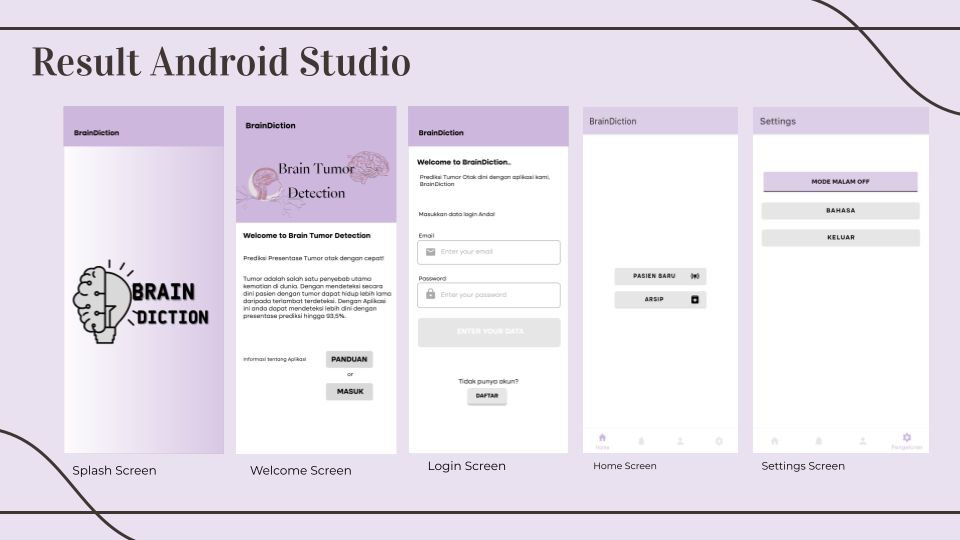
\includegraphics[scale=0.35]{./assets/loginhome}
	\caption{Tampilan login dan beranda aplikasi.}
\end{figure}
\begin{figure}[H]
	\centering
	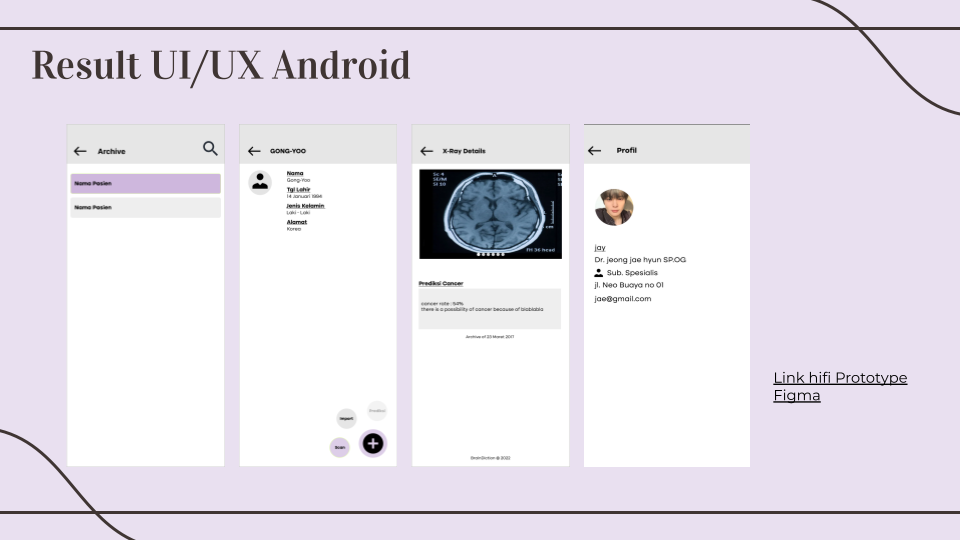
\includegraphics[scale=0.35]{./assets/predictionscreen}
	\caption{Tampilan prediksi aplikasi.}
\end{figure}
\subsection{Implementasi Materi}
Pada produk ini, kelompok kami mengimplementasikan seluruh elemen \textit{learning path} pada program Bangkit 2022:
\begin{enumerate}
	\item \textit{Cloud Computing} pada Google Cloud Platform
	\begin{itemize}
		\item Google Firebase Authentication
		\item Google Cloud Run untuk \textit{Backend} aplikasi dan \textit{machine learning}
		\item Google Cloud SQL untuk penyimpanan data pasien dan data prediksi
	\end{itemize}
	\item \textit{Machine Learning}
	\begin{itemize}
		\item Tensorflow untuk training model pendeteksi tumor otak
		\item Flask untuk \textit{Backend} penyalur dari Cloud Run ke model yang dihasilkan
	\end{itemize}
	\item \textit{Android Development}
	\begin{itemize}
		\item Kotlin dan Figma untuk pembuatan UI/UX aplikasi
	\end{itemize}
\end{enumerate}
% Daftar Pustaka
\selectlanguage{english}
%\printbibliography[title={DAFTAR PUSTAKA}]

	
\end{document}